\section{Aula 17 de Outubro de 2019}
\label{2019_10_17}

% #region continuação teo5 caso ->infty
\subsection*{\it Continuação}

\begin{teorema}
  \normalfont\textbf{[T5.]}
  Seja
  \vspace*{-\baselineskip}
  \[
    p = \nicefrac{1}{n}\left(\log n + c_n\vphantom{1j}\right)
  \]
  então
  \vspace*{-\baselineskip}
  \[
    \lim_{n\rightarrow\infty} \mathds{P}\left(G\left(n,\ p\vphantom{1j}\right) \text{ é conexo}\vphantom{1j}\right) = \left\{\begin{array}{ll}
      0                               & \text{se } c_n\rightarrow-\infty                            \\
      \mathrel{e}^{-\mathrel{e}^{-c}} & \text{se } c_n\rightarrow c\in\mathds{R}                        \\
      1                               & \text{se } c_n\rightarrow\infty                             \\
    \end{array}\vphantom{1j}\right.
  \]
\end{teorema}

Seja $X_k=\#$componentes de $G\left(n,\ p\vphantom{1j}\right)$ com $k$ vértices.

Por exemplo, $X_1=\#$vértices isolados.

\begin{proof}[Prova caso $c_n\rightarrow\infty$]
  $ $\newline
  Temos
  \vspace*{-\baselineskip}
  \begin{align*}
    \mathds{P}\left(G\left(n,\ p\vphantom{1j}\right)\text{ é desconexo}\vphantom{1j}\right)
      &=    \mathds{P}\left(\sum_{1\leq k\leq\nicefrac{n}{2}}X_k\geq 1\vphantom{1j}\right)
      \leq  \mathds{E}\left(\sum_{1\leq k\leq\nicefrac{n}{2}}\vphantom{1j}\right)                                                     \\
      &=    \sum_{1\leq k\leq\nicefrac{n}{2}}\mathds{E}\left(X_k\vphantom{1j}\right)
      \leq  \sum_{1\leq k\leq\nicefrac{n}{2}}\binom{n}{k}\left(1-p\vphantom{1j}\right)^{k\left(n-k\vphantom{1j}\right)}
  \end{align*}

  Também temos
  \begin{align*}
    \sum_{1\leq k\leq n^{\nicefrac{3}{4}}}\binom{n}{k}\left(1-p\vphantom{1j}\right)^{k\left(n-k\vphantom{1j}\right)}
      &\leq \sum_{1\leq k\leq n^{\nicefrac{3}{4}}}\left(\nicefrac{\mathrm{e} n}{k}\cdot\mathrm{e}^{-p\left(n-k\vphantom{1j}\right)}\vphantom{1j}\right)^k                  \\
      &\leq \sum_{1\leq k\leq n^{\nicefrac{3}{4}}}
              \left(\nicefrac{\mathrm{e} n}{k}\cdot\mathrm{e}^{-\log n-c_n+\smash{\overbrace{2\nicefrac{k}{n}\log n}^{o(1)}}}\vphantom{1j}\right)^k    \\
      &\leq \sum_{1\leq k\leq n^{\nicefrac{3}{4}}}\left(\nicefrac{2}{k}\cdot\mathrm{e}^{1-c_n}\vphantom{1j}\right)^k
      \leq  3\mathrm{e}^{1-c_n} 
      \rightarrow 0
  \end{align*}

  Ademais,
  \begin{align*}
    \sum_{n^{\nicefrac{3}{4}}<k\leq\nicefrac{n}{2}}\binom{n}{k}\left(1-p\vphantom{1j}\right)^{k\left(n-k\vphantom{1j}\right)}
      &\leq \sum_{n^{\nicefrac{3}{4}}<k\leq\nicefrac{n}{2}}
              \left(\mathrm{e}\cdot\smash{\overbrace{\nicefrac{n}{k}}^{<n^{\nicefrac{1}{4}}}}\cdot
              \mathrm{e}^{\smash{\overbrace{-p\left(n-k\vphantom{1j}\right)}^{\geq\nicefrac{n}{2}}}}\vphantom{1j}\right)^k                             \\
      &\leq \sum_{n^{\nicefrac{3}{4}}<k\leq\nicefrac{n}{2}}\left(\mathrm{e}\cdot n^{\nicefrac{1}{4}}\cdot\mathrm{e}^{\nicefrac{-\log n}{2}}\vphantom{1j}\right)^k
      \leq  n^{\nicefrac{1}{5}\cdot n^{\nicefrac{3}{4}}}
      \rightarrow 0
  \end{align*}
\end{proof}
% #endregion

% #region comentários sobre teo5 caso ->c
\clearpage
\subsection*{\normalfont Comentários sobre o caso $c_n\rightarrow c\in\mathds{R}$.}$ $\newline

Podemos usar
\vspace*{-\baselineskip}
\[
  \mathds{E}\left(X_k\vphantom{1j}\right) = \binom{n}{k} \left(1-p\vphantom{1j}\right)^{k\left(n-k\vphantom{1j}\right)} k^{k-2} p^{k-1}
\]

Pelo Teorema de Cayley [<\href{https://en.wikipedia.org/wiki/Cayley%27s_formula}{https://en.wikipedia.org/wiki/Cayley\%27s\_formula}>: \#árvores geradoras de ordem $n$, temos que
\[
  k^{k-2} p^{k-1} = p\left(k\,p\vphantom{1j}\right)^{k-2} \rightarrow 0 \text{ se } k>2
\]

Segue que no outro caso caso $c_n\rightarrow c$
\[
  \mathds{P}\left(\sum_{k=2}^{\nicefrac{n}{2}} X_k \geq 1\vphantom{1j}\right) = \mathds{E}\left(\sum_{k=2}^{\nicefrac{n}{2}} X_k\vphantom{1j}\right) \rightarrow 0
\]

Concluímos que, com prob. $\rightarrow1$, $G\left(n,\ p\vphantom{1j}\right)$ é composto por uma componente e $X_1$ vértices isolados.

Assim, $G\left(n,\ p\vphantom{1j}\right)$ é conexo se e só se $X_1=0$.

Vale que $X_1$ converge em probabilidade para uma v.a. $\mathrm{Pois}\left(\mathrm{e}^{-c}\vphantom{1j}\right)$.

Distribuição \textbf{Poison} [<\href{https://en.wikipedia.org/wiki/Poisson_distribution}{https://en.wikipedia.org/wiki/Poisson\_distribution}>]:
\begin{itemize}
  \item $Z\sim\mathrm{Pois}\left(\lambda\vphantom{1j}\right)$;
  \item $Z\in\mathds{N}$;
  \item $\mathds{P}\left(Z=t\vphantom{1j}\right) = \mathrm{e}^{-\lambda}\cdot\nicefrac{\lambda^t}{t!}$, $t>0$;
  \item $\mathds{E}\left(Z\vphantom{1j}\right) = \lambda$; e 
  \item $\mathds{P}\left(Z=0\vphantom{1j}\right) = \mathrm{e}^{-c}$.
\end{itemize}

Lembrando que $\mathds{E}\left(X_1\vphantom{1j}\right)\rightarrow\mathrm{e}^{-c}$:
\[
  \lim_{n\rightarrow\infty} \mathds{P}\left(X_1=t\vphantom{1j}\right)
    = \mathds{P}\left(\mathrm{Pois}\left(\mathrm{e}^{-c}\vphantom{1j}\right)=t\vphantom{1j}\right)
    = \mathrm{e}^{-\mathrm{e}^{-c}}\,\nicefrac{\left(\mathrm{e}^{-c}\vphantom{1j}\right)^t}{t!}
\]

Para todo $t$ fixo. Em particular,
\[
  \mathds{P}\left(G\left(n,\ p\vphantom{1j}\right) \text{ é conexo}\vphantom{1j}\right) = \lim_{n\rightarrow\infty} \mathds{P}\left(X_1=0\vphantom{1j}\right)=\mathrm{e}^{-\mathrm{e}^{-c}}
\]
%endregion

% #region teoB-Th87
\clearpage
\subsection{Teorema de Bollubón e Thomson}$ $\newline

[\textit{Primeiro teorema para qualquer propriedade crescente. Antes, era preciso provar para cada uma.}]

[\textit{Prova original era com teoria dos conjuntos, mais complicada.}]

\begin{teorema}
  \normalfont\textbf{[T6 B-Th'87.]}
  Seja $\mathcal{P}$ uma propriedade não trivial crescente. Então $\mathcal{P}$ admite uma função limiar:
  \vspace*{-\baselineskip}
  \begin{align*}
    \mathds{P}\left(G_p\in\mathcal{P}\vphantom{1j}\right)
      &\rightarrow \left\{\begin{array}{ll}
                      0 & \text{se } p \ll p_0  \\
                      1 & \text{se } p \gg p_0  \\
                    \end{array}\vphantom{1j}\right.                                                                  \\
    \mathds{P}\left(G_p\not\in\mathcal{P}\vphantom{1j}\right)
      &\leq\epsilon
  \end{align*}
\end{teorema}

\begin{proof}[(Esboço)]$ $\newline
  Seja $p_0<p_0\left(n\vphantom{1j}\right)$ tal que
  \vspace*{-\baselineskip}
  \[
    \mathds{P}\left(G\left(n,\ p\vphantom{1j}\right)\in\mathcal{P} = \nicefrac{1}{2}\vphantom{1j}\right)
  \]

  Fixe $\epsilon>0$, e seja $t$ t.q. $\left(\nicefrac{1}{2}\vphantom{1j}\right)t\leq\epsilon$. Considere $t$ cópias independentes de $G\left(n,\ p\vphantom{1j}\right)$, digamos $G_1,\ \ldots,\ G_t$. Seja $p'$ t.q. $1-p'=(1-p_0)^t$. Temos
  \[
    G\left(n,\ p'\vphantom{1j}\right) = G_1\cup\ldots\cup G_t
  \]

  Temos que
  \vspace*{-\baselineskip}
  \[
    \mathds{P}\left(G\left(n,\ p\vphantom{1j}\right)\not\in\mathcal{P}\vphantom{1j}\right)
      \leq \prod_{1\leq i\leq t} \mathds{P}\left(G_i\not\in\mathcal{P}\vphantom{1j}\right)
      = \left(\nicefrac{1}{2}\vphantom{1j}\right)^t
      \leq \epsilon
  \]

  Segue que se $p\gg p_0$, então
  \[
    \mathds{P}\left(G\left(n, p\vphantom{1j}\right)\not\in\mathcal{P}\vphantom{1j}\right) \rightarrow 0
  \]

  Um argumento análogo prova que se $p\ll p_0$, então
  \[
    \mathds{P}\left(G\left(n, p\vphantom{1j}\right)\in\mathcal{P}\vphantom{1j}\right) \rightarrow 0
  \]
\end{proof}
% #endregion

% #region transição de fase em GNP
\clearpage
\subsection{Transição de fase em $G(n,\ p)$}$ $\newline

[$G_t\approx G\left(n,\ \nicefrac{t}{\binom{n}{2}}\vphantom{1j}\right)$, $t=p\binom{n}{2}\sim p\,\nicefrac{n^2}{2}$, $p=\nicefrac{1}{n}$.]

[Propriedades crescente têm uma transição tipo $\left[a\,p,\ b\,p\vphantom{1j}\right]$, com $a\rightarrow0$ e $b\rightarrow\infty$.]

Seja $L_k\left(G\vphantom{1j}\right)=$\#vértices da $k$-ésima maior componente de $G$. Claro que $L_1\left(G\vphantom{1j}\right)\geq L_1\left(G\vphantom{1j}\right)\geq\ldots$.

\begin{teorema}
  \normalfont\textbf{[T7.]}
  Seja $\epsilon>0$ uma constante fixa.
  \begin{enumerate}
    \item Se $p=\nicefrac{\left(1-\epsilon\vphantom{1j}\right)}{n}$, então q.c. $G\left(n,\ p\vphantom{1j}\right)$ é t.q. $L_1\left(G\left(n,\ p\vphantom{1j}\right)\vphantom{1j}\right)\leq c\,\log n$, onde $c=c_\epsilon$.
    \item Se $p=\nicefrac{\left(1+\epsilon\vphantom{1j}\right)}{n}$, então q.c. $G\left(n,\ p\vphantom{1j}\right)$ é t.q. $L_1\left(G\left(n,\ p\vphantom{1j}\right)\vphantom{1j}\right)\geq c\,n$ e $L_2\left(G\left(n,\ p\vphantom{1j}\right)\vphantom{1j}\right)\leq c\,\log n$, onde $c=c_\epsilon$.
  \end{enumerate}
\end{teorema}

\begin{proof}[Prova]$ $\newline
  Vamos provar que se $p=\nicefrac{\left(1+\epsilon\vphantom{1j}\right)}{n}$, então $L_1\left(G\left(n,\ p\vphantom{1j}\right)\vphantom{1j}\right)\geq\nicefrac{1}{24}\,\epsilon^2\,n$ com prob. $\rightarrow1$.

  Usamos busca em profundidade:
  \begin{enumerate}
    \item $U\leftarrow V=V\left(G\vphantom{1j}\right)$;
    \item $G=G\left(n,\ p\vphantom{1j}\right)$;
    \item $E\leftarrow\varnothing$;
    \item $F\leftarrow\varnothing$; e
    \item Para cada $v\in V$, se $v\in U$ então $\texttt{dfs}\left(v\vphantom{1j}\right)$.
  \end{enumerate}
\end{proof}

\begin{itemize}[label={}]
  \item $\texttt{dfs}\left(v\vphantom{1j}\right)$
  \begin{itemize}[label={}]
    \item $F\leftarrow F\cup\left\{v\vphantom{1j}\right\}$
    \item $U\leftarrow U\setminus\left\{v\vphantom{1j}\right\}$
    \item Para cada $w\neq v$
    \begin{itemize}[label={}]
      \item se $w\in U$
      \item então se $\left\{v,\ w\vphantom{1j}\right\}\in\mathds{E}\left(G\left(n,\ p\vphantom{1j}\right)\vphantom{1j}\right)$ (query)
      \begin{itemize}[label={}]
        \item $\texttt{dfs}\left(w\vphantom{1j}\right)$
      \end{itemize}
    \end{itemize}
    \item $E\leftarrow E\cup\left\{v\vphantom{1j}\right\}$
    \item $F\leftarrow F\setminus\left\{v\vphantom{1j}\right\}$
  \end{itemize}
\end{itemize}

Executamos a $\texttt{dfs}$ até fazermos $t=\delta\,n^2$ queries, onde $\delta=\nicefrac{\epsilon}{4}$.

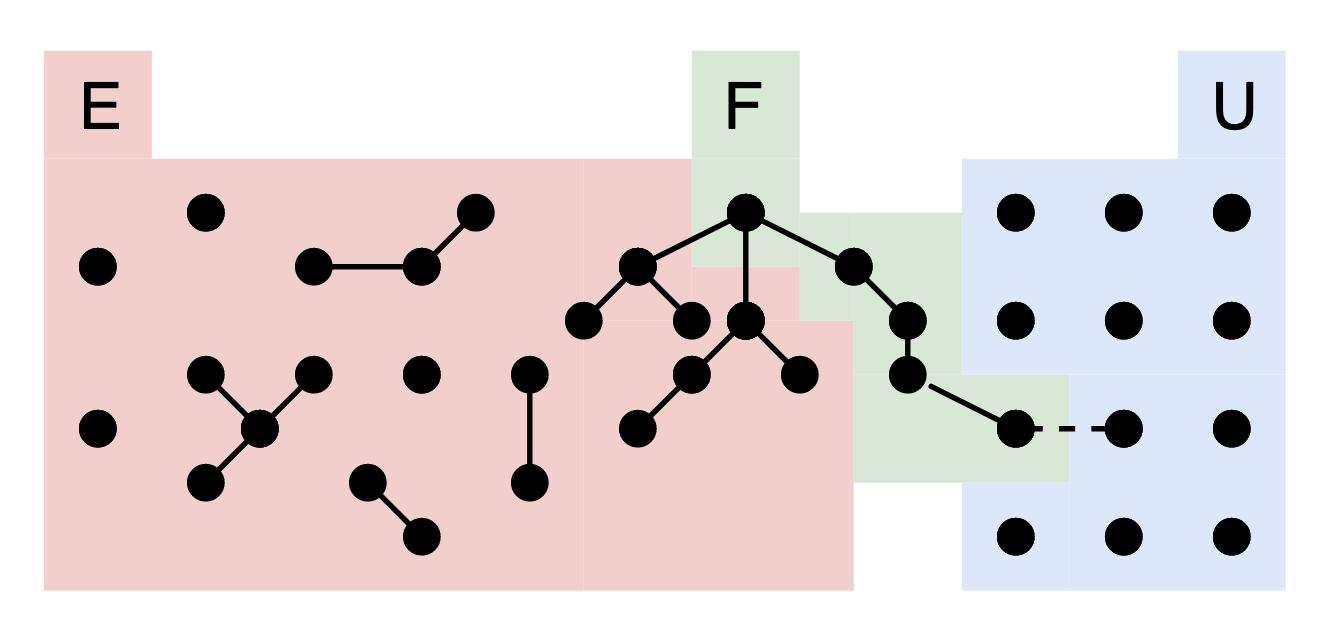
\includegraphics[width=0.75\textwidth]{aulas/10_17/dfs.png}

\begin{observacao}
  O valor esperado de queries com resposta positiva é $\delta\,n^2\,p=\delta\left(1+\epsilon\vphantom{1j}\right)$. Com prob. $\rightarrow1$, temos que o número de respostas positivas é t.q.
  \[
    \delta\left(1+\nicefrac{\epsilon}{2}\vphantom{1j}\right)n \leq s \leq \delta\left(1+2\,\epsilon\vphantom{1j}\right)n
  \]
  
  Por Chebyshev ou Chernoff.
  
  Sem perda de generalidade, $\epsilon\leq\nicefrac{1}{4}$.
\end{observacao}

\begin{fato}
  \normalfont
  $\not\exists$ arestas  em $G\left(n,\ p\vphantom{1j}\right)$ entre $E$ e $U$.
\end{fato}

Provamos que, se $L_1\left(G\left(n,\ p\vphantom{1j}\right)\vphantom{1j}\right)<\nicefrac{1}{24}\,\epsilon^2\,n$, então $\left|E\vphantom{1j}\right|\,\left|U\vphantom{1j}\right|>t$.

Isso é uma contradição.

Vamos provar que, em algum momento, $\left|F\vphantom{1j}\right|\geq\nicefrac{1}{24}\,\epsilon^2\,n$, c.c. $\left|E\vphantom{1j}\right|\,\left|U\vphantom{1j}\right|>t$.
% #endregion


